%%\documentclass[12pt,russianb]{report}
%\usepackage[russian]{babel}
%\usepackage[cp1251]{inputenc}


\documentclass{report}
\usepackage[T2A]{fontenc}
\usepackage[utf8]{inputenc}
\usepackage[english,russian]{babel}

\usepackage{longtable}   % подключение длинных таблиц
\usepackage[dvipsnames]{xcolor}
\usepackage{multirow}
\usepackage{array}
\usepackage{indentfirst} % идентификация первых абзацев после секционирования
\usepackage{lastpage}    % пакет достчета страниц 

\usepackage{fancyhdr}                    % расширенный формат страниц
\voffset=-25mm   % -25                   % сдвиг страницы вверх
\hoffset=-15mm   % -10     


  \usepackage[pdftex]{graphicx}            % загрузка графики под pdf
  \usepackage{cmap}                        % чтоб работал поиск по PDF 
  \usepackage[unicode, pdftex, colorlinks, linkcolor=blue]{hyperref}   % гиперссылки в PDF
  \pdfcompresslevel=9                      % сжимаем PDF 
  \textheight=240mm                        % для PDF высота печатного текста
  \textwidth=165mm                         % ширина печатного текста
  \renewcommand{\baselinestretch}{1.3}        % для PDF интервалы между
  \baselineskip=1.3\baselineskip              % строками 


\pagestyle{empty}
\pagestyle{fancy}
\lhead{\tiny ООО <<Опти-Софт>>}
\chead{}
\rhead{\tiny Отчет по обследованию производства \FIRMA}
\cfoot{\rule{\textwidth}{0.25pt}
~\arabic{page}}

\sloppy                             % подавление дополнительных переносов
\righthyphenmin=2                   % можно переносить
\setlength{\parindent}{10mm}        % отступ красной строки

\usepackage{todonotes}
%\newcommand{\todo}[1]{}
%\renewcommand{\todo}[1]{{\color{red} TODO: {#1}}}



\usepackage{placeins}    % пакет позволяет вставлять плавающие объекты (рисунки) в том месте, 
                         % где это необходимо. Для вывода рисунка после него встаить команду \FloatBarrier
                         
                         
                         

\newcommand{\red}[1]{\textcolor{Red}{#1}}
\newcommand{\green}[1]{\textcolor{Green}{#1}}
\newcommand{\blue}[1]{\textcolor{Blue}{#1}}                       
\newpage

\subsection{Управление взаимоотношениями с клиентами}
\label{BP_CRM}

Поиском новых клиентов занимаются менеджеры отдела продаж.

Менеджеры ищут новых клиентов в различных открытых источниках, через обзвон потенциальных покупателей, через Интернет, систему 2Gis.
Менеджеры для поиска новых клиентов используют холодные звонки, выставки.

% Для продаж выделено 4 менеджера и 2 инженера по отгрузке.

CRM системы не выявлено.
Новых клиентов каждый менеджер ведет в своих файлах, блокнотах. Единой базы потенциальных покупателей не выявлено.

Новых клиентов бухгалтер заводит в справочник Контрагенты в системе 1С:УПП только при заключении договора.


В отделе продаж работает шесть человек: старший, ведущий, младший менеджер.
Выделено три группы менеджеров. Реально создано только две группы.

% Новые клиенты заносятся как лиды. МАП заносит карточку покупателя в модуле CRM системы 1С: УНФ. МАП ведет историю взаимоотношений с клиентами вручную записывая историю звонков, рассылок.
% В CRM созданы шаблоны сценариев работы с покупателем. Каждое событие работы с контрагентом является  элементом справочника с тем  шаблоном.
% При появлении потенциального клиента МАП определяет лицо принимающее решение со стороны организации. МАП запрашивает требования по изготовлению изделия и получает техническое задание (размеры и характеристики нового изделия). 

% В отделе продаж есть четкий регламент работы по новым заказчикам.
% Одна сделка представляет собой несколько изделий готовой продукции для одного клиента.



Опросного листа по клиенту не выявлено.
%
Общего списка потенциальных клиентов и холодных клиентов не выявлено.
Старший менеджер ведет таблицу в Excel по потенциальным клиентам (форма \ref{pic:d3}).
%
%
%
%%
%Учет взаимоотношений с клиентами ведется на ручном уровне. Менеджеры отдела маркетинга 
%занимаются поиском и привлечением новых покупателей. Выделяется пассивный поиск через сайт, рекламу и участие в мероприятиях, и активный поиск через адресную рассылку.
%Все контакты хранятся на сетевом ресурсе в сети ПРЕДПРИЯТИЯ, куда есть доступ большинству пользователей сети.
%При появлении нового покупателя менеджеры отдела маркетинга создают каталог в сетевом каталоге клиентов.
%Внутри каталога хранится информация по письмам с клиентами, договорам, спецификациям и тендерам.
%
%%
%Новых заказчиков ведет менеджер отдела продаж и закупок.
%После выполнения предварительных заказов заказчику ведущий специалист отдела продаж передает клиентов менеджерам отдела продаж.
%%
%%\begin{figure}
%%\begin{center}
%%\ifnum\pdfoutput=0
%%  \includegraphics[40,0][366,292]{Pics/TK1.png}
%%\else 
%%  \includegraphics[height=0.94\textheight, keepaspectratio]{Pics/CustomerList.jpg}
%%\fi
%%\end{center}
%%  \caption{Разделение потребителей гофротары в разрезе маркетологов}
%%  \label{pic:CustomerList}
%%\end{figure}
%%\clearpage
%%
%%
\begin{figure}
\begin{center}
 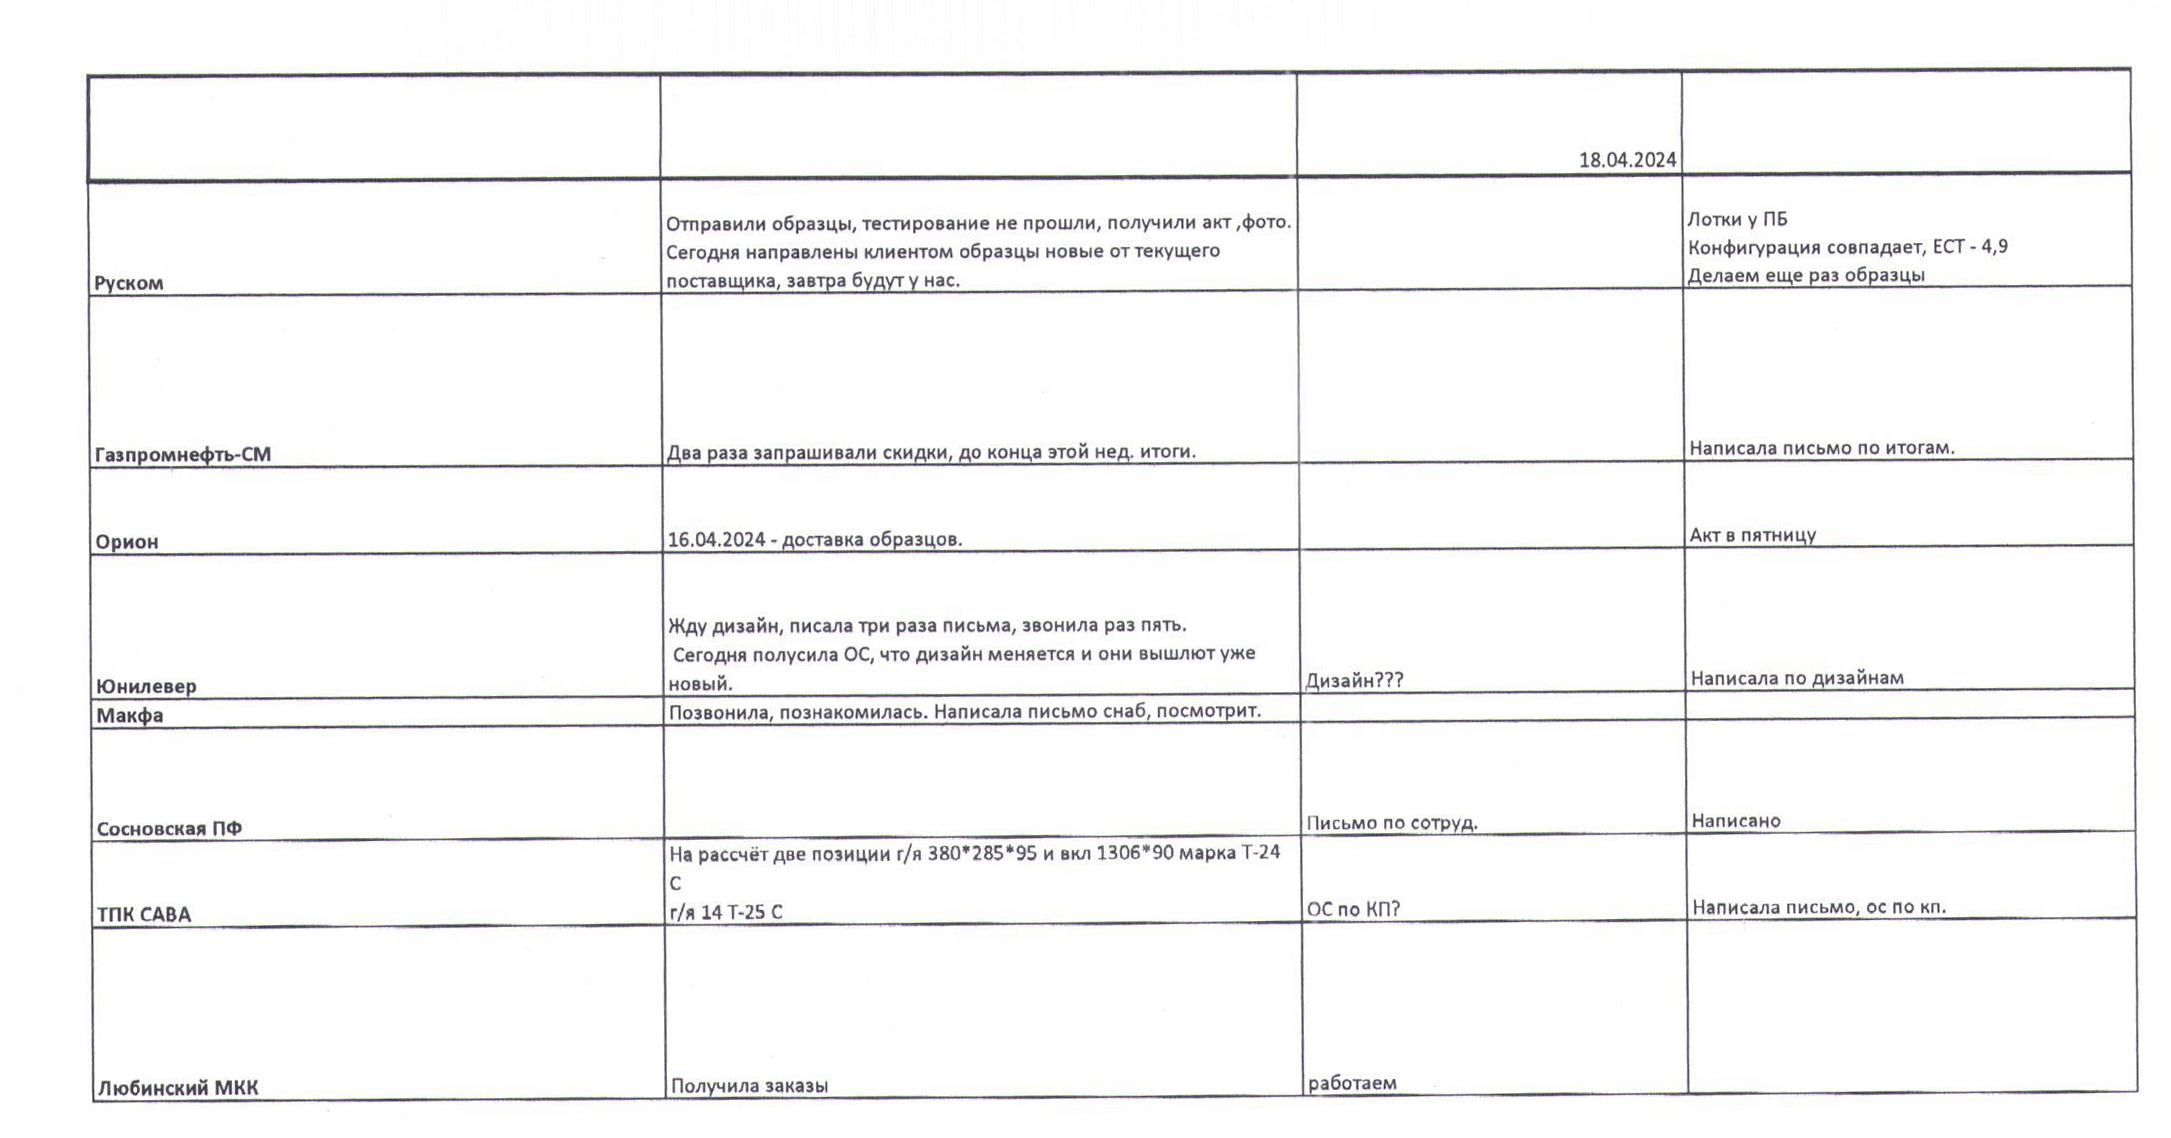
\includegraphics[height=0.5\textheight, angle=90, keepaspectratio]{Pics/d03.jpg}
\end{center}
 \caption{Список потенциальных покупателей}
 \label{pic:d3}
\end{figure}
\clearpage
%
%


\clearpage
\ifx \notincludehead\undefined
\normalsize
\end{document}
\fi 